\chapter{Code và Demo}
\label{chap:code}

\section{Cấu trúc mã nguồn}

\begin{code}{Cấu trúc thư mục chính của project}
\label{lst:tree}
\begin{minted}{text}
MultiAgent/
├── app.py                        FastAPI: API + phục vụ giao diện
├── docker-compose.yml            neo4j, qdrant, seaweedfs, backend, cloudflared
├── src/
│   ├── communication/
│   │   ├── message_bus.py        AgentMessage, BaseAgent, MessageBus (định tuyến + audit trail)
│   │   └── summary.py            tóm tắt một dòng cho mỗi thông điệp (cho Phòng hội chẩn)
│   ├── agents/                   9 agent: orchestrator, conversation, document, clarification,
│   │                             prediction, knowledge, consensus_critic, treatment_rl, response
│   ├── models/                   tabular_ml (GBDT), deep_mlp (PyTorch), rnn_temporal, qlearning_treatment
│   ├── knowledge/                ingest (tạo KB), embedder, clinical_criteria (ngưỡng ADA), scope
│   ├── storage/
│   │   ├── db.py, models.py      SQLite (SQLAlchemy) + bảng ảo FTS5
│   │   ├── vector_store.py       QdrantVectorStore: tìm kiếm lai Qdrant + FTS5, RRF
│   │   └── graph_store.py        Neo4jGraphStore: MERGE bộ ba, duyệt lân cận bằng Cypher
│   └── api/                      routes_chat, routes_session, routes_system, routes_lab
├── scripts/                      fetch_nhanes, fetch_brfss (3,17 triệu người), train_model,
│                                 ingest_kb, chat_cli
├── data/kb_sources/              10 tài liệu ADA 2024 / QĐ 5481 + curated_triples.json
├── frontend/src/components/      MainChat, ConsultationDetails, AgentRoom (Phòng hội chẩn)
└── tests/                        43 kiểm thử tự động
\end{minted}
\end{code}

\section{Các hàm chính}

\begin{table}[H]
\centering
\caption{Các hàm và lớp chính}
\label{tab:functions}
\small
\begin{tabularx}{\linewidth}{@{}L{5.2cm}Y@{}}
\toprule
\textbf{Hàm / lớp} & \textbf{Vai trò} \\
\midrule
\texttt{MessageBus.send} & Ghi thông điệp, định tuyến tới agent nhận, chuyển ngoại lệ thành \texttt{FAILURE}, đo thời gian xử lý \\
\texttt{OrchestratorAgent.run\_turn} & Phân loại ý định, lập kế hoạch, chạy song song các nhánh, trả về câu trả lời và transcript \\
\texttt{PredictionAgent.handle} & Dự đoán bằng GBDT + MLP; trả lời ba loại chất vấn \\
\texttt{QdrantVectorStore.hybrid\_search} & Truy vấn Qdrant và FTS5, gộp bằng RRF, đọc nội dung đoạn từ SQLite \\
\texttt{Neo4jGraphStore.neighborhood} & GraphRAG: duyệt lân cận 1–2 bước từ các thực thể, trả về cạnh kèm \texttt{chunk\_ids} \\
\texttt{ConsensusCriticAgent.handle} & Phát hiện mâu thuẫn, tranh biện nhiều vòng, phân tầng, guardrail \\
\texttt{TreatmentRLAgent.handle} & Chọn hành động theo Q-table rồi áp luật ràng buộc \\
\texttt{ingest\_documents}, \texttt{rebuild\_graph} & Tạo KB: SQLite + Qdrant + Neo4j \\
\texttt{AgentRoom} (React) & Phát lại transcript trên sơ đồ agent \\
\bottomrule
\end{tabularx}
\end{table}

\begin{code}{MessageBus: các agent không gọi hàm của nhau (\texttt{src/communication/message\_bus.py}, rút gọn)}
\label{lst:bus}
\begin{minted}{python}
async def send(self, msg: AgentMessage) -> AgentMessage:
    self._record(msg)                                   # audit trail theo conversation
    agent = self.agents.get(msg.receiver)
    if agent is None or msg.msg_type not in agent.handles:
        reply = failure(msg, "NOT_UNDERSTOOD")
    else:
        try:
            reply = await agent.handle(msg)
        except Exception as exc:                        # lỗi một agent không làm sập hội đồng
            reply = agent.reply(msg, f"{msg.msg_type}_FAILED", {"error": str(exc)},
                                performative="FAILURE")
    reply.elapsed_ms = int((time.perf_counter() - started) * 1000)
    self._record(reply)
    return reply
\end{minted}
\end{code}

\begin{code}{Tìm kiếm lai Qdrant + SQLite FTS5 (\texttt{src/storage/vector\_store.py}, rút gọn)}
\label{lst:hybrid}
\begin{minted}{python}
def _fts_ranked(self, query_text, limit):
    words = _words(query_text)                          # bỏ dấu câu và từ hư tiếng Việt
    match = " OR ".join(f'"{w}"' for w in words)
    return self.session.execute(text(
        "SELECT rowid, -bm25(kb_chunks_fts, 3.0, 1.0) FROM kb_chunks_fts "
        "WHERE kb_chunks_fts MATCH :q ORDER BY bm25(kb_chunks_fts, 3.0, 1.0) LIMIT :n"),
        {"q": match, "n": limit}).all()

def hybrid_search(self, query_text, query_vec, k=5, pool=30):
    vec = self.client.query_points(self.collection, query=query_vec, limit=pool).points
    fused = _rrf([(p.id, p.score) for p in vec], self._fts_ranked(query_text, pool), k + 5)
    return self._attach(fused)[:k]                      # nối nội dung đoạn văn từ SQLite
\end{minted}
\end{code}

\section{Cách chạy}

\begin{code}{Cài đặt và chạy hệ thống}
\label{lst:run}
\begin{minted}{bash}
cp .env.example .env                                  # GEMINI_API_KEY không bắt buộc
docker compose up -d neo4j qdrant seaweedfs           # SQLite là file, không cần container
python3 -m venv .venv && .venv/bin/pip install -r requirements.txt
.venv/bin/python scripts/fetch_nhanes.py              # tải NHANES vào SQLite
.venv/bin/python scripts/fetch_brfss.py               # BRFSS 2011–2023: 3.172.819 người (~740 MB)
.venv/bin/python scripts/train_model.py               # huấn luyện GBDT + MLP trên NHANES và BRFSS
.venv/bin/python scripts/ingest_kb.py                 # tạo KB: SQLite + Qdrant + Neo4j
.venv/bin/python -m uvicorn app:app --port 8000       # http://localhost:8000
.venv/bin/python -m pytest -q                         # 43 kiểm thử
docker compose --profile app up -d --build            # triển khai toàn bộ + Cloudflare Tunnel
\end{minted}
\end{code}

Khi chạy, có thể xem đồ thị tri thức trực tiếp trên Neo4j Browser (\texttt{http://localhost:7474}) và các vector trên Qdrant Dashboard (\texttt{http://localhost:6333/dashboard}).

\section{Demo: chatbot và Phòng hội chẩn}

Giao diện là một chatbot web (React). Người dùng nhập tin nhắn tự do, nói bằng giọng, hoặc đính kèm phiếu xét nghiệm. Để người xem \emph{thấy} được hệ đa agent đang làm việc, giao diện có thêm panel \textbf{Phòng hội chẩn} bên phải (\figref{fig:ui-full}):
\begin{itemize}
  \item \textbf{Sơ đồ agent} bố trí theo đúng sơ đồ của đề bài: Dự đoán (DB → ML + DL) ở trên, Tri thức (Neo4j KB + RAG) ở dưới, Hội đồng (+/−) bên phải, Can thiệp (RL + luật) ở góc dưới, tầng tiếp nhận bên trái, Điều phối ở giữa.
  \item \textbf{Phát lại từng thông điệp}: mỗi bước vẽ một mũi tên từ agent gửi tới agent nhận, có chấm sáng chạy dọc theo cung, màu theo performative (xanh dương \texttt{REQUEST}, xanh lá \texttt{INFORM}, đỏ \texttt{CHALLENGE}, cam \texttt{RESPONSE}). Agent đang nói được viền sáng; agent chưa tham gia bị làm mờ.
  \item \textbf{Bong bóng phát biểu}: câu tóm tắt nội dung thông điệp, ví dụ ``Mô hình và xét nghiệm đang nói khác nhau — anh giải thích thế nào?''.
  \item \textbf{Điều khiển}: phát, tạm dừng, tua từng bước, thanh trượt, đổi tốc độ; danh sách toàn bộ thông điệp bấm được để nhảy tới.
  \item Mỗi câu trả lời trong khung chat có nút ``Xem các tác tử phối hợp'' để mở lại đúng lượt hội chẩn đó.
\end{itemize}

\begin{figure}[H]
\centering
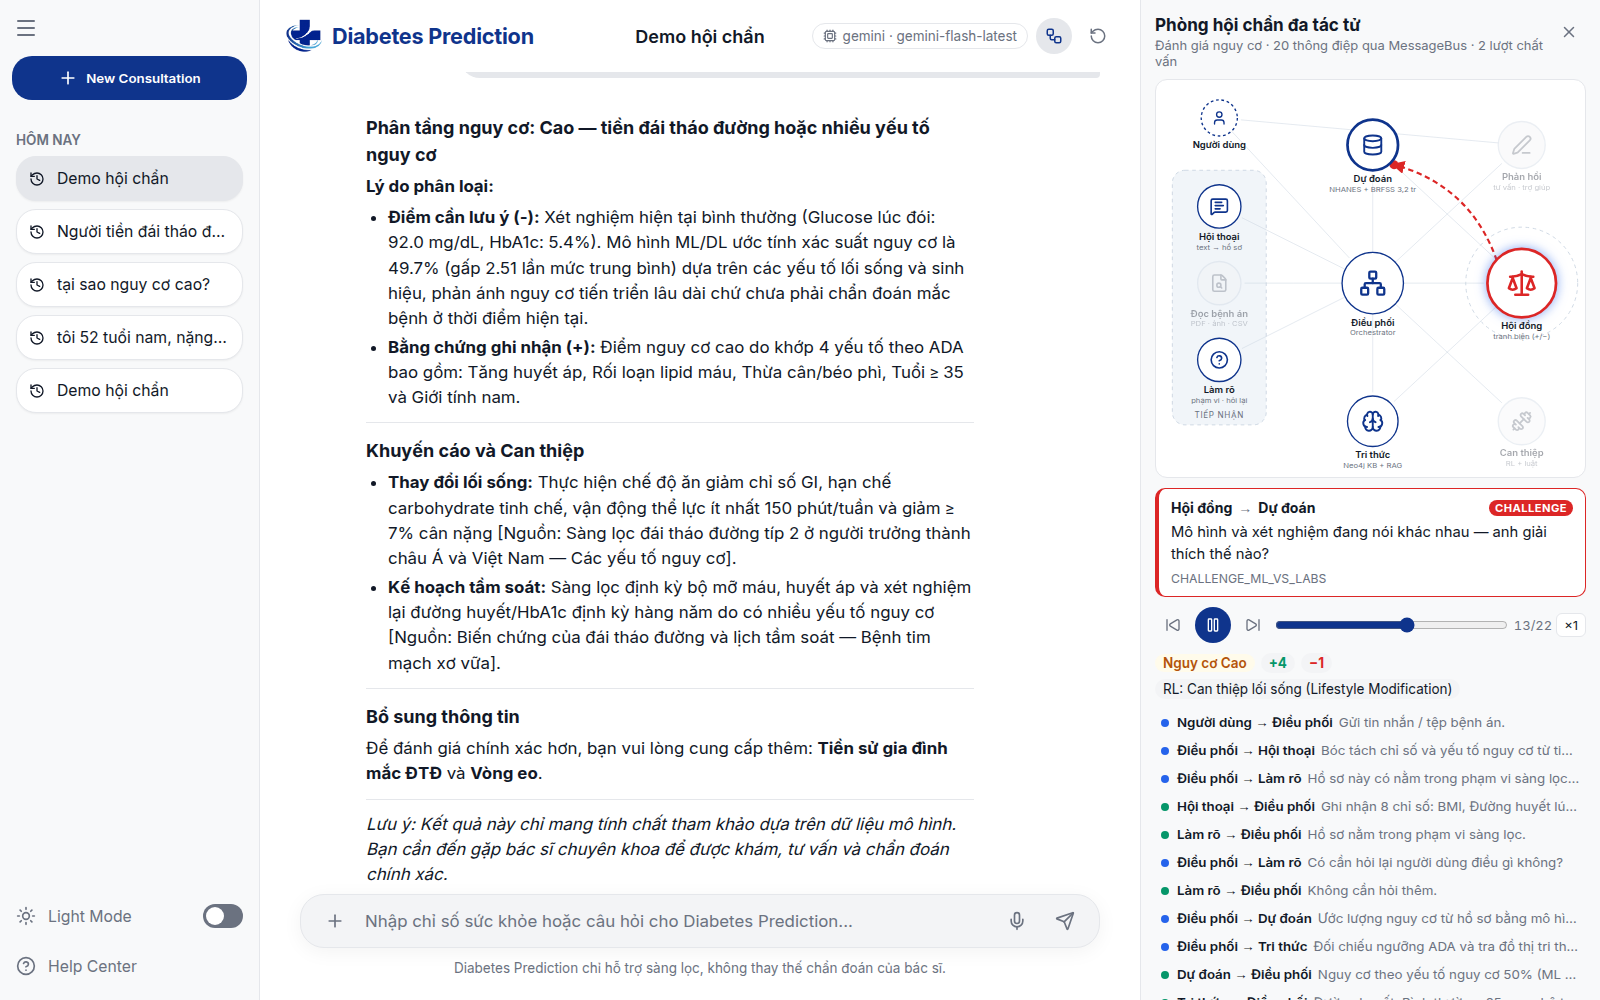
\includegraphics[width=\linewidth]{ui_debate.png}
\caption{Giao diện chatbot và Phòng hội chẩn: hội đồng đang chất vấn agent Dự đoán (mũi tên đỏ)}
\label{fig:ui-full}
\end{figure}

\begin{figure}[H]
\centering
\begin{minipage}[t]{0.32\linewidth}\centering
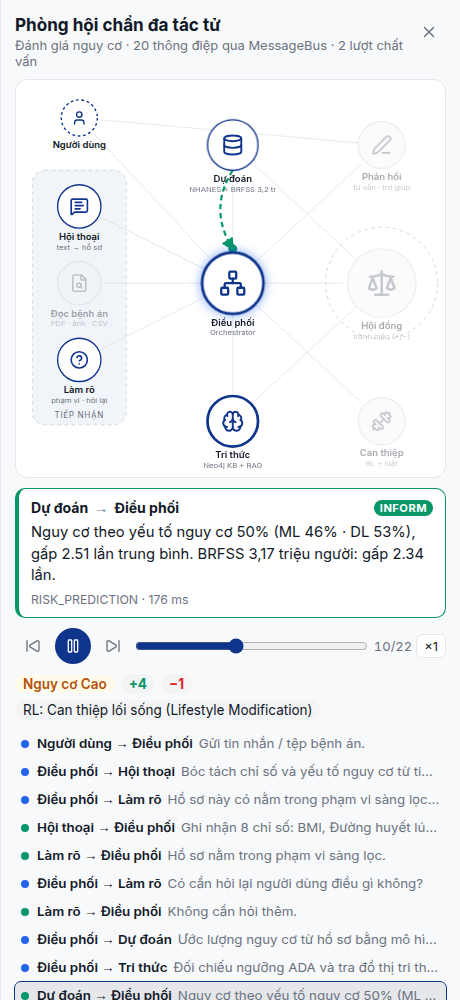
\includegraphics[width=\linewidth,trim=0 380 0 0,clip]{ui_branches_room.png}\\[-2pt]{\footnotesize (a) Nhánh DL trả kết quả}
\end{minipage}\hfill
\begin{minipage}[t]{0.32\linewidth}\centering
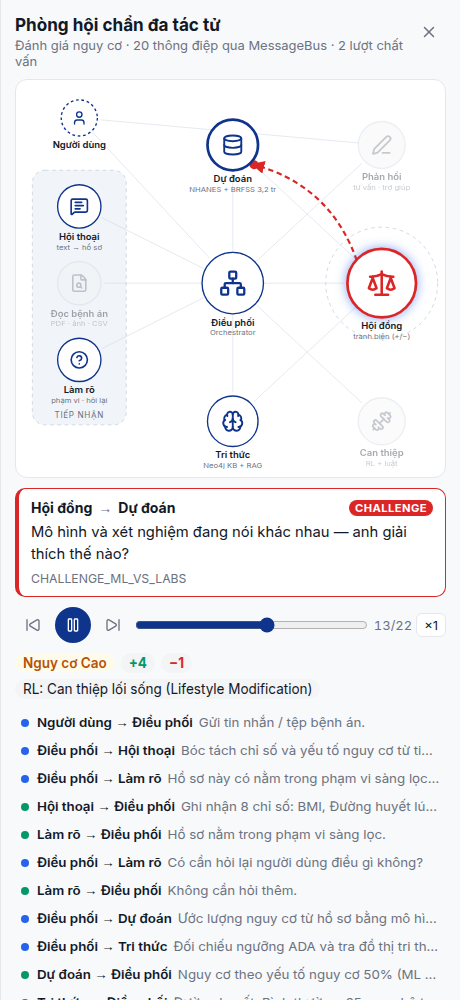
\includegraphics[width=\linewidth,trim=0 380 0 0,clip]{ui_debate_room.png}\\[-2pt]{\footnotesize (b) Hội đồng chất vấn}
\end{minipage}\hfill
\begin{minipage}[t]{0.32\linewidth}\centering
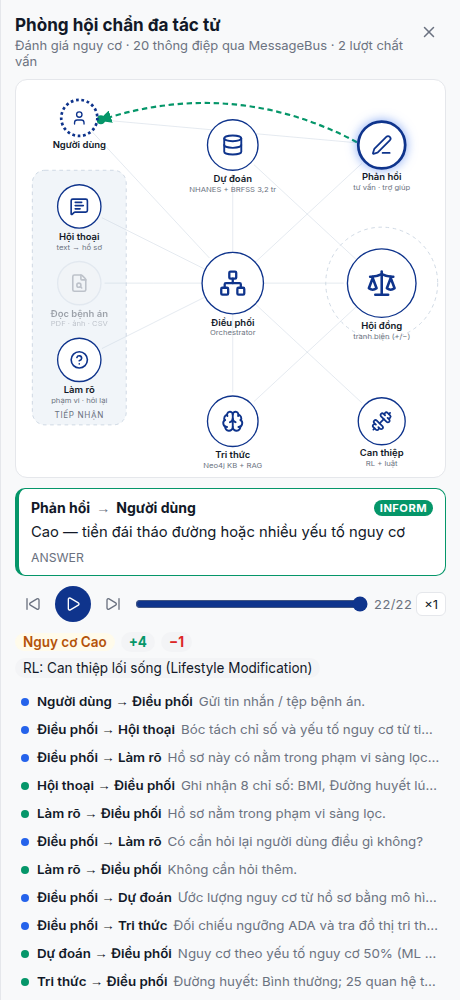
\includegraphics[width=\linewidth,trim=0 380 0 0,clip]{ui_final_room.png}\\[-2pt]{\footnotesize (c) Trả lời người dùng}
\end{minipage}
\caption{Ba thời điểm khi phát lại một lượt hội chẩn trong Phòng hội chẩn}
\label{fig:ui-steps}
\end{figure}

\subsection*{Khối ``Hội đồng đang suy luận'' trong khung chat}

Ngoài Phòng hội chẩn, phần suy luận còn hiện \emph{ngay trong khung chat} theo thời gian thực, giống cách các trợ lý AI hiển thị quá trình suy nghĩ. Endpoint \api{POST /api/chat/stream} trả về luồng NDJSON: \texttt{MessageBus} đẩy mỗi thông điệp ra ngay khi ghi nhận (qua một \texttt{ContextVar} gắn với lượt chat, nên các nhánh chạy song song bằng \texttt{asyncio.gather} cũng được đẩy ra). Khi agent Tri thức duyệt Neo4j, backend gửi thêm một sự kiện \texttt{graph} chứa đúng các nút và cạnh vừa đi qua, và giao diện vẽ ngay đồ thị đó: nút xuất phát ở giữa, nút cách 1 bước ở vòng trong, 2 bước ở vòng ngoài, tô màu theo nhãn ontology (\figref{fig:ui-thinking}a). Suy luận xong, khối tự thu gọn thành một dòng tóm tắt; người dùng bấm vào mới mở lại các bước và đồ thị (\figref{fig:ui-thinking}b).

\begin{figure}[H]
\centering
\begin{minipage}[t]{0.5\linewidth}\centering
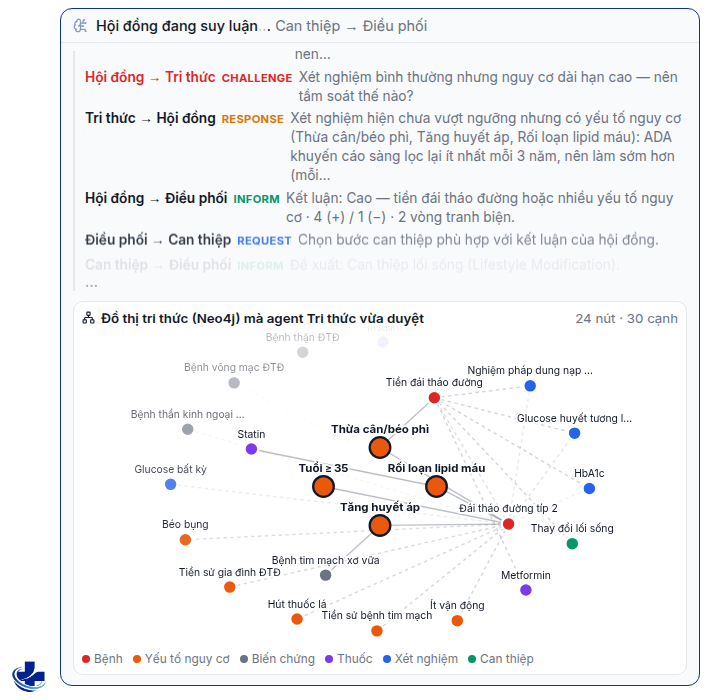
\includegraphics[width=\linewidth]{ui_thinking_live.png}\\[-2pt]{\footnotesize (a) Đang suy luận: từng thông điệp và đồ thị Neo4j vừa duyệt}
\end{minipage}\hfill
\begin{minipage}[t]{0.47\linewidth}\centering
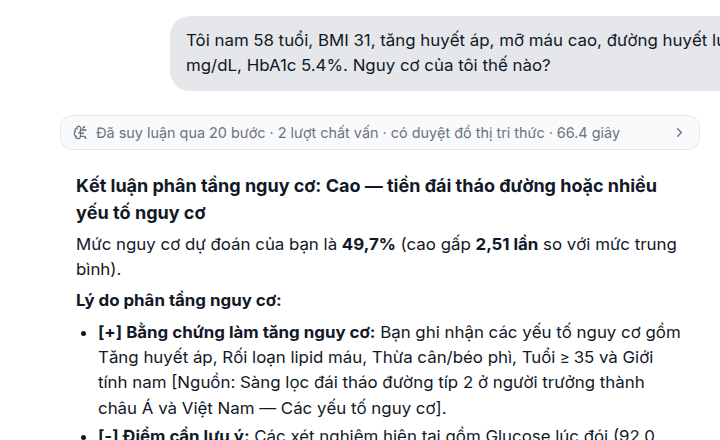
\includegraphics[width=\linewidth]{ui_thinking_done.png}\\[-2pt]{\footnotesize (b) Xong: thu gọn thành dropdown phía trên câu trả lời}
\end{minipage}
\caption{Khối suy luận của hội đồng trong khung chat}
\label{fig:ui-thinking}
\end{figure}

\section{Ví dụ một lượt hội chẩn}

Tin nhắn demo: ``Tôi nam 58 tuổi, BMI 31, tăng huyết áp, mỡ máu cao, đường huyết lúc đói 92 mg/dL, HbA1c 5.4\%. Nguy cơ của tôi thế nào?''. Đây là ca điển hình gây mâu thuẫn: xét nghiệm \emph{bình thường} nhưng yếu tố nguy cơ \emph{dày đặc}. Hệ thống chạy ở chế độ không LLM. \tabref{tab:transcript} là toàn bộ 22 thông điệp mà MessageBus ghi lại, kèm câu tóm tắt hiển thị trong Phòng hội chẩn.

\begin{table}[H]
\centering
\caption{Luồng 22 thông điệp của lượt hội chẩn demo (ms: thời gian xử lý ở thông điệp trả lời)}
\label{tab:transcript}
\scriptsize
\begin{tabularx}{\linewidth}{@{}r L{2.0cm} L{2.0cm} L{1.5cm} Y r@{}}
\toprule
\textbf{\#} & \textbf{Gửi} & \textbf{Nhận} & \textbf{Perf.} & \textbf{Nội dung (tóm tắt)} & \textbf{ms} \\
\midrule
1–2 & Orchestrator $\rightleftarrows$ & Conversation & REQ / INF & Ghi nhận 6 chỉ số: FPG, HbA1c, BMI, tuổi, tăng huyết áp, rối loạn mỡ máu & 3 \\
3–6 & Orchestrator $\rightleftarrows$ & Clarification & REQ / INF & Hồ sơ nằm trong phạm vi sàng lọc; không cần hỏi thêm & 0 \\
7, 9 & Orchestrator $\rightleftarrows$ & Prediction & REQ / INF & NHANES: nguy cơ 47\% (ML 45\% · DL 50\%), gấp 2,38 lần trung bình; BRFSS 3,17 triệu người: gấp 2,43 lần & 232 \\
8, 10 & Orchestrator $\rightleftarrows$ & Knowledge & REQ / INF & Đường huyết bình thường; 25 quan hệ trên đồ thị tri thức & 1.260 \\
11 & Orchestrator & Critic & REQUEST & Mở hội đồng: tổng hợp bằng chứng và tranh biện & \\
12 & Critic & Prediction & \textbf{CHALLENGE} & Hồ sơ còn thiếu nhiều đặc trưng — dự đoán còn tin được không? & \\
13 & Prediction & Critic & RESPONSE & Mới có 31\% đặc trưng; mô hình được huấn luyện cho dữ liệu thiếu, hạ độ tin cậy & 0 \\
14 & Critic & Prediction & \textbf{CHALLENGE} & Mô hình và xét nghiệm nói khác nhau — giải thích thế nào? & \\
15 & Prediction & Critic & RESPONSE & Mô hình không dùng glucose nên phản ánh nguy cơ tiến triển; đồng ý xét nghiệm là căn cứ chẩn đoán, đề nghị giữ tầm soát & 0 \\
16 & Critic & Knowledge & \textbf{CHALLENGE} & (vòng 2) Xét nghiệm bình thường nhưng nguy cơ dài hạn cao — tầm soát thế nào? & \\
17 & Knowledge & Critic & RESPONSE & ADA: sàng lọc lại ít nhất mỗi 3 năm, sớm hơn khi nhiều yếu tố nguy cơ; giảm cân, vận động 150 phút/tuần & 22 \\
18 & Critic & Orchestrator & INFORM & Kết luận: Cao — 5 (+) / 2 (−), 2 vòng tranh biện; có (+) ``mô hình quy mô lớn đồng thuận'' & 23 \\
19–20 & Orchestrator $\rightleftarrows$ & TreatmentRL & REQ / INF & Đề xuất: can thiệp lối sống (luật giới hạn vì xét nghiệm chưa ở ngưỡng ĐTĐ) & 0 \\
21–22 & Orchestrator $\rightleftarrows$ & Response & REQ / INF & Viết câu trả lời có trích dẫn & 0 \\
\bottomrule
\end{tabularx}
\end{table}

Ví dụ này cho thấy giá trị của tranh biện. Một hệ thống chỉ dùng ngưỡng sẽ trả lời ``đường huyết bình thường''. Một hệ thống chỉ dùng mô hình sẽ trả lời ``nguy cơ 47\%'' mà không giải thích vì sao xét nghiệm lại bình thường. Hội đồng đưa cả hai góc nhìn ra, hòa giải chúng thành một kế hoạch tầm soát có trích dẫn, và cho người dùng thấy cả điểm đồng thuận lẫn điểm còn cần lưu ý (hồ sơ còn thiếu giới tính, vòng eo, huyết áp, tiền sử gia đình). Hai mô hình huấn luyện trên hai quần thể khác nhau (20 nghìn người có xét nghiệm và 3,17 triệu người tự khai) cho nguy cơ tương đối gần như trùng nhau (2,38 và 2,43 lần), nên hội đồng ghi thêm một bằng chứng (+) độc lập. Toàn bộ phần ``suy nghĩ'' của hội đồng mất khoảng 1,3 giây, phần lớn là nhánh Tri thức trong lần gọi đầu (nạp mô hình nhúng và duyệt đồ thị).

\section{Kiểm thử}

\begin{table}[H]
\centering
\caption{Bộ kiểm thử tự động (43 kiểm thử, đều đạt)}
\label{tab:tests}
\small
\begin{tabularx}{\linewidth}{@{}L{4.4cm}Y@{}}
\toprule
\textbf{Tệp} & \textbf{Nội dung} \\
\midrule
\texttt{test\_clinical\_criteria.py} & Ngưỡng ADA cho FPG, HbA1c, OGTT; quy tắc ``2 kết quả bất thường'' \\
\texttt{test\_extraction.py} & Trích chỉ số từ tin nhắn tiếng Việt, quy đổi đơn vị, đọc PDF, ảnh, DOCX, CSV \\
\texttt{test\_scope.py} & Phát hiện hồ sơ ngoài phạm vi và kế hoạch câu hỏi làm rõ \\
\texttt{test\_large\_scale.py} & Hội đồng chỉ chất vấn khi mô hình NHANES và BRFSS nằm ở hai phía ngược nhau; phản hồi hạ độ tin cậy \\
\texttt{test\_summary.py} & Câu tóm tắt cho từng loại thông điệp trong Phòng hội chẩn \\
\texttt{test\_multi\_agent.py} & Cả hội đồng chạy trên SQLite + Qdrant + Neo4j: hỏi lại khi thiếu dữ liệu, tranh biện 2 vòng, câu hỏi kiến thức không chạy nhánh dự đoán, guardrail ghi đè, câu hỏi tiếp nối trả lời từ bộ nhớ \\
\bottomrule
\end{tabularx}
\end{table}

\section{Đánh giá đầu–cuối}

Hệ thống được đánh giá trên \textbf{400 ca} lấy ngẫu nhiên từ tập kiểm tra NHANES (\agent{PredictionAgent} chưa từng thấy), chỉ giữ người có cả FPG và HbA1c: 23,0\% mắc ĐTĐ. Đánh giá chạy không LLM để kết quả tất định, trên đúng bộ lưu trữ SQLite + Qdrant + Neo4j của project.

\begin{table}[H]
\centering
\caption{Đủ xét nghiệm (FPG + HbA1c): tính đúng đắn và vận hành của hội đồng (399 ca)}
\label{tab:k1}
\small
\begin{tabularx}{\linewidth}{@{}L{5.6cm}Y@{}}
\toprule
\textbf{Chỉ số} & \textbf{Kết quả} \\
\midrule
Phân loại đường huyết đúng ngưỡng ADA & \textbf{399/399 (100\%)} \\
Áp đúng quy tắc ``2 xét nghiệm bất thường'' & \textbf{71/71 (100\%)} \\
Dữ liệu ngoài miền sinh lý & 1 ca BMI 74,8 bị từ chối, hệ thống hỏi lại thay vì dự đoán \\
Số vòng tranh biện & 0 vòng: 288 ca · 1 vòng: 100 · 2 vòng: 11 \\
Chất vấn được mở & xác minh tiêu chí 71 · ML–DL bất đồng 30 · ML thấp nhưng xét nghiệm ĐTĐ 13 · ML cao nhưng xét nghiệm bình thường 11 → lịch tầm soát 11 · \textbf{NHANES–BRFSS bất đồng 10} \\
Mô hình quy mô lớn (BRFSS) & cùng phía với mô hình chính ở 97,5\% ca; trung bình 4,6 điểm (+) mỗi ca (3,7 khi chưa có BRFSS) \\
Safety Guardrail & ưu tiên 77 ca · khám sớm 11 ca \\
Gợi ý can thiệp (RL sau ràng buộc) & lối sống 358 · metformin 5 · phối hợp tim–thận 25 · chuyên khoa 11 \\
Thông điệp mỗi lượt & 16–22 (trung bình 16,7); 146 cặp CHALLENGE/RESPONSE \\
Độ trễ một lượt (không LLM) & trung vị 136 ms, p95 192 ms; Prediction 129 ms (4 mô hình + giải thích) ‖ Knowledge 73 ms chạy song song \\
\bottomrule
\end{tabularx}
\end{table}

\figw[0.95\linewidth]{ch7_ops}{Thời gian xử lý của từng agent và tần suất các loại chất vấn}

\begin{table}[H]
\centering
\caption{Chỉ có FPG: giá trị của việc phối hợp nhiều agent (399 ca, 91 người ĐTĐ)}
\label{tab:k2}
\small
\begin{tabular}{@{}lccccr@{}}
\toprule
\textbf{Cách ra quyết định} & \textbf{Độ nhạy} & \textbf{Đặc hiệu} & \textbf{PPV} & \textbf{F1} & \textbf{Số ca dương} \\
\midrule
Agent Tri thức đơn lẻ: FPG ≥ 126 & 0,582 & \textbf{1,000} & \textbf{1,000} & \textbf{0,736} & 53 \\
Agent Tri thức đơn lẻ: FPG ≥ 100 & 0,879 & 0,520 & 0,351 & 0,502 & 228 \\
Agent Dự đoán đơn lẻ: ML ≥ 30\% & 0,659 & 0,841 & 0,551 & 0,600 & 109 \\
\textbf{Hội đồng: mức Cao hoặc Rất cao} & \textbf{0,945} & 0,458 & 0,340 & 0,500 & 253 \\
\bottomrule
\end{tabular}
\end{table}

\figw[0.95\linewidth]{ch7_k2}{Độ nhạy, đặc hiệu của các cách ra quyết định, và tỉ lệ ĐTĐ thật theo mức nguy cơ của hội đồng}

\textbf{Nhận xét.} Hai agent đơn lẻ bỏ sót những nhóm khác nhau. Ngưỡng FPG ≥ 126 chính xác tuyệt đối nhưng chỉ bắt được 58\% người ĐTĐ: 38 người ĐTĐ có FPG dưới 126 (đang điều trị tốt, hoặc chỉ có HbA1c vượt ngưỡng). Hội đồng kết hợp xét nghiệm với mô hình đạt \textbf{độ nhạy 0,945}, bắt thêm \textbf{33/38} ca mà FPG bỏ sót. Điểm nguy cơ của hội đồng có AUC 0,876, cao hơn FPG đơn lẻ (0,862) và mô hình đơn lẻ (0,855). Cái giá là độ đặc hiệu 0,46. Đây là đánh đổi có chủ đích của một công cụ \emph{sàng lọc}: mức Cao nghĩa là ``nên làm thêm HbA1c hoặc OGTT'', một xét nghiệm rẻ, trong khi bỏ sót người bệnh thì đắt hơn nhiều. Phân tầng có ý nghĩa rõ: mức Rất cao 100\% là ĐTĐ thật (53/53), mức Thấp chỉ 1,6\% (2/128).

Với tin nhắn tiếng Việt tự do sinh từ mẫu câu (399 tin), bộ trích xuất regex lấy đúng 100\% các trường, và 91\% tin nhắn cho cùng mức nguy cơ như khi nhập form. Phần còn lại khác mức vì tin nhắn ngẫu nhiên lược bớt thông tin (vòng eo, huyết áp, tiền sử), chứ không phải do trích sai.

\section{Hạn chế và hướng phát triển}

\begin{itemize}
  \item \textbf{Mô hình}: trên NHANES, MLP chỉ nhỉnh hơn hồi quy logistic; cả hai bộ dữ liệu là của Hoa Kỳ, chưa hiệu chỉnh cho người Việt. BRFSS bổ sung 14.249 người gốc Á ở tập kiểm tra (AUC 0,85) nhưng có nhãn tự khai, bỏ sót người mắc chưa được chẩn đoán, nên chỉ dùng làm ý kiến thứ hai.
  \item \textbf{RAG}: embedding MiniLM yếu với tiếng Việt chuyên ngành, làm tìm kiếm lai kém hơn toàn văn đơn lẻ trên bộ 60 câu. Hướng sửa: đổi sang E5 đa ngôn ngữ (hit@3 0,98 trong thí nghiệm của tiểu luận) hoặc gán trọng số cho RRF; mở rộng KB và bộ câu hỏi đánh giá.
  \item \textbf{RL}: môi trường và hàm thưởng tự đặt, chưa học từ dữ liệu điều trị thật. Hướng phát triển: mô phỏng đường huyết theo giờ để agent học kế hoạch ăn uống và vận động hằng ngày.
  \item \textbf{Trích xuất không LLM}: regex còn bỏ sót một số cách viết, ví dụ ``Tôi nam 58 tuổi'' chưa nhận ra giới tính trong ca demo. Khi có LLM, phần này do Gemini đảm nhận.
  \item \textbf{Đánh giá}: số liệu tin nhắn tự do là cận trên lạc quan, vì tin nhắn sinh từ mẫu câu mà regex được viết để hiểu.
\end{itemize}
